\chapter{Mint}\label{mint}

Prior to the development of the summarization system, it was important to develop a sense for what is needed from such a system, and what problems can it solve. To answer these quesitons, I developed an Aeolus application based on the financial management service \emph{mint.com}. The \emph{Mint} application served as a case study and guided the development of the summarization system.

In this chapter I present the Mint application model as well as some examples to how a summarization system could be used for this application.

\section{Mint Model}

Mint.com is an financial management service that provides its users with the ability to monitor their bank accounts across different banks from one place. It also allows users to run transaction analysis tools that will access the information of certain transactions for each bank for the user, and generate a result. In addition, Mint runs aggregate analysis for all user accounts.

For example, Bob could sign up on www.mint.com and add his Bank of America account and his US Bank account for monitoring. This will cause our application to store credentials for both of these banks for Bob. Bob can then request a graph that presents his expenditures on food in the last week. Bob's actions would also affect the general aggregate analysis done over all Mint users.

This example gives us a starting idea of how should we build our authority structure. For instance, there should be a \emph{BOB-DATA} tag associated with Bob's information (e.g. expenditure statistics, transactions, etc.) that only a principal running on Bob's behalf can declassify. Note that Bob's password should never be revealed to Bob himself, neither should any of Bob's bank credential be revealed as well. Furthermore, there's a natural grouping of user data tags, and hence a super tag, \emph{ALL-USER-DATA}, could be useful to run the aggregate analysis tools for Mint.

In this section we examine the security model of the application more closely.

\subsection{Authority State Model}

\begin{figure}[h]
\centering
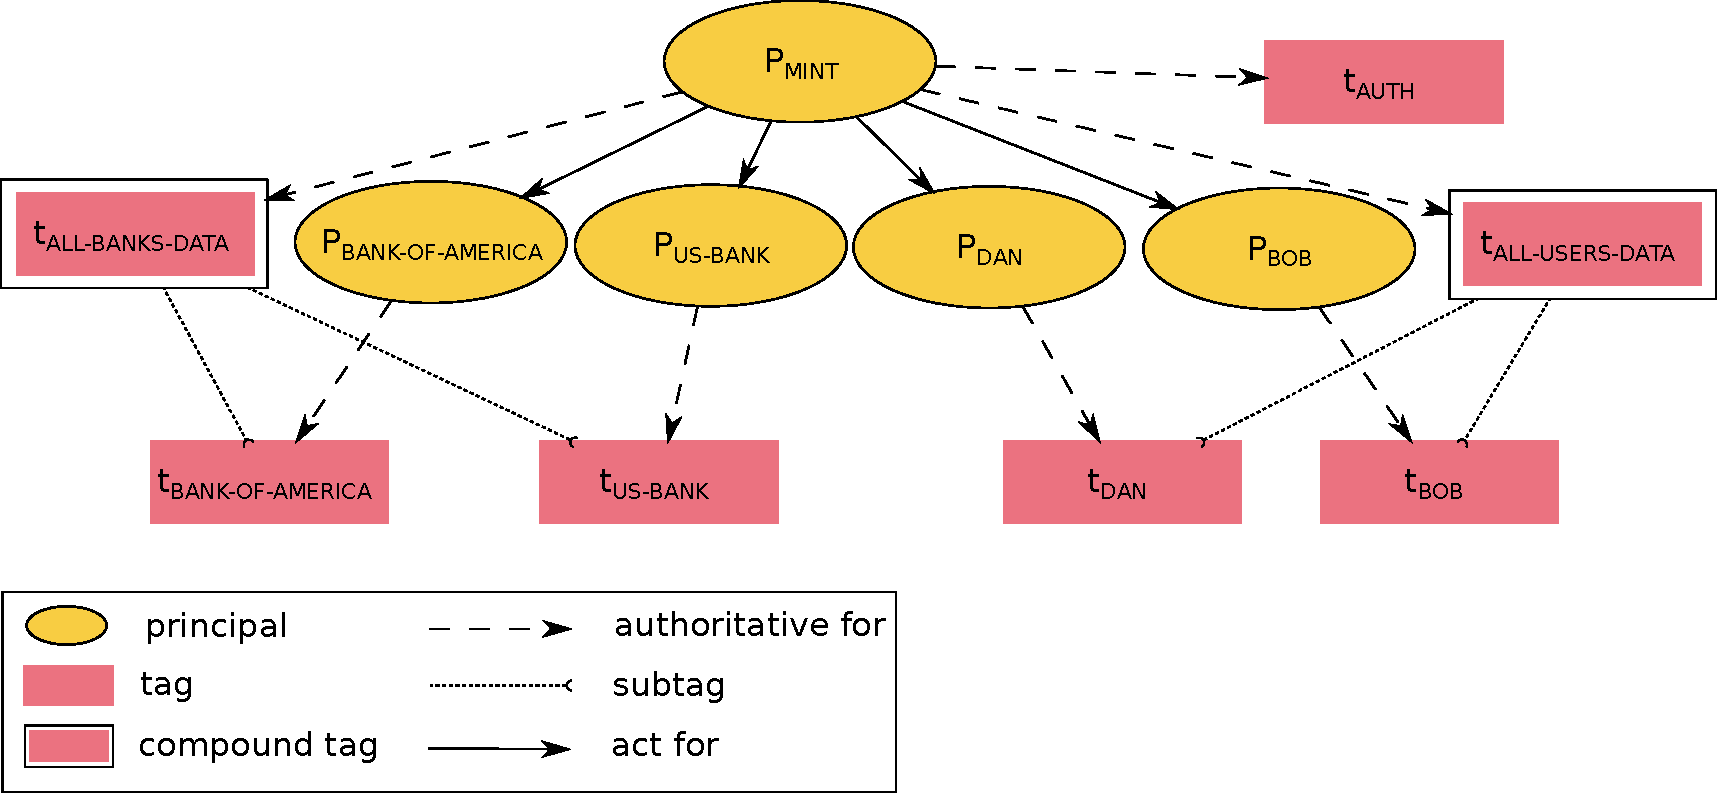
\includegraphics[width=\textwidth,height=\textheight,keepaspectratio]{figures/mint-auth-state-model}
\caption{Mint Authority State Model. In this example, two banks are registered at the application: Bank of America and US Bank. Users Bob and Dan have both signed up. Principals are denoted \emph{P$_{<name>}$} and tags are denoted \emph{t$_{<name>}$}.}
\label{fig:mint-auth-state-model}
\end{figure}


In this section we identify the prinicpals running in the system, the tags associated with different data, and the relationships between them. Figure \ref{fig:mint-auth-state-model} shows an overview of the authority state model for Mint.

An intuitive way to list all necessary\footnote{Neccessary by good design. The application could run with just one principal.} principals, is to think of the different ``clearance levels'' in the system: some information should be accessible by a user, some by a bank, and some information should not be accessible at all. In the light of these requirements, the application employs the following principals:
\begin{description}
  \item[Mint principal] \ \\
    This principal is authoritative for all tags in the system, and is
    used for aggregate analysis of user data and
    user authentication.
  \item[Bank principals] \ \\
    Each of these principals is authoritative for a particular bank's tag.
  \item[User principals] \ \\
    Each of these principals is authoritative for a particular user's tag.
  \item[Public principal] \ \\
    Described in section \ref{aeolus:auth-calls}, this
    principal is used when no privileged operations are 
    necessary to ensure no information leaks.
\end{description}

Similarly, to separate data in the system according to its purpose, (e.g. user password, credentials to download bank transactions, etc..), the application employs the following tags:
\begin{description}
  \item[User data tags] \ \\
    Each of these tags is associated with data 
    carrying a particular user's information.
    Reading (or modifying) user information
    requires declassifying (or endorsing)
    a user data tag.
  \item[Bank data tags] \ \\
    Each of these tags is associated 
    with data carrying a particular bank's information.
    Reading a user's bank credentials
    requires declassifying a bank data tag. This tag is
    important so that only a Bank's closure is able
    to access a user's bank password.
  \item[All-Users-Data tag] \ \\ 
    This tag is a super tag for all the user 
    tags.
    Running aggregate analysis on Mint user accounts
    requires declassifying this tag.
  \item[All-Banks-Data tag] \ \\ 
    This tag is a super tag for all the bank tags.
    Adding a new bank to Mint requires endorsing
    this tag.
  \item[Authentication tag] \ \\
    This tag is associated with user's Mint passwords.
    Authenticating a user's mint credentials
    requires declassifying this tag.
    This tag is important to prevent release of
    a user's password to someone who might have
    gained access to their account.
\end{description}

The following two sections explain how data is stored in the system and which tag operations are carried out in a typical workflow.

\subsection{Files}\label{sec:mint-fs}

\begin{figure}[h]
\centering
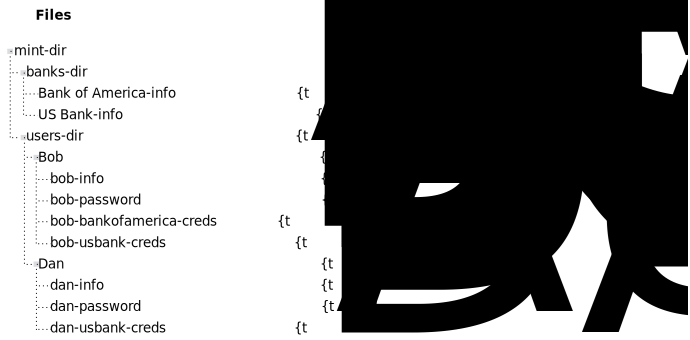
\includegraphics[width=\textwidth,height=\textheight,keepaspectratio]{figures/mint-filesystem}
\caption{The file system hierarchy for Mint. In continuation of the example in figure \ref{fig:mint-auth-state-model}, Bob added accounts in both banks to his Mint account, and Dan added a US BANK account to his Mint account.Tags are shown under the secrecy label and integrity label columns, and are denoted \emph{t$_{<name>}$}. \emph{t$_{BOB}$} and \emph{t$_{DAN}$} are both \emph{USER-DATA} tags.}
\label{fig:mint-fs}
\end{figure}

The application uses Aeolus files for persistent storage. Figure \ref{fig:mint-fs} shows the hierarchy of the Mint files and their labels, described below:
%The application stores it's information under a root directory called \emph{mint-dir}.  The are two direct subdirectories of \emph{mint-dir}: \emph{banks-dir} and \emph{users-dir}.

\begin{description}
  \item[\emph{mint-dir}] \ \\
    This is the root directory for the Mint 
    application.
    The secrecy label is empty, the integrity 
    label contains the \emph{ALL-USERS-DATA}, 
    \emph{ALL-BANKS-DATA} and 
    \emph{ALL-USERS-AUTH} tags.
  \begin{description}
    \item[\emph{banks-dir}] \ \\
      Contains a \emph{bank-info} file for each 
      bank that was registered to the 
      application. This 
      directory has an empty secrecy label, and 
      has the \emph{ALL-BANKS-DATA} tag in its 
      integrity labels.
      Each of the \emph{bank-info} files in 
      this directory has a \emph{BANK-DATA} 
      tag in both its secrecy and integrity 
      labels.
    \item[\emph{users-dir}] \ \\
      Has the \emph{ALL-USER-DATA} tag in both 
      its secrecy and integrity labels. Contains 
      a subdirectory per user, each subdirectory 
      contains a \emph{USER-DATA} tag in its 
      secrecy label, and a \emph{USER-DATA} tag 
      in its integrity label.
      Each of these subdirectories contains the 
      following files:
      \begin{description}
        \item[\emph{user-info}] \ \\
          Contains the user tag for that user.
          This file has the \emph{USER-DATA} tag 
          in both its secrecy and integrity labels.
        \item[\emph{user-password}] \ \\
          Contains the user's password.
          This file contains the \emph{AUTH} tag in 
          its secrecy label, and the \emph{USER-DATA} 
          tag in its integrity label.
        \item[\emph{user-bank-creds}] \ \\
          Contains user credentials for a particular 
          bank.
          The \emph{users-dir} directory contains 
          one \emph{user-bank-creds} file per bank 
          the user added to their account.
          This file has the \emph{BANK-DATA} and 
          \emph{USER-DATA} tags in its secrecy label, 
          and the \emph{USER-DATA} tag in its 
          integrity label.
      \end{description}
  \end{description}
\end{description}

\subsection{Shared Memory Objects}
\label{sec:mint-smo}

\begin{figure}[h]
\centering
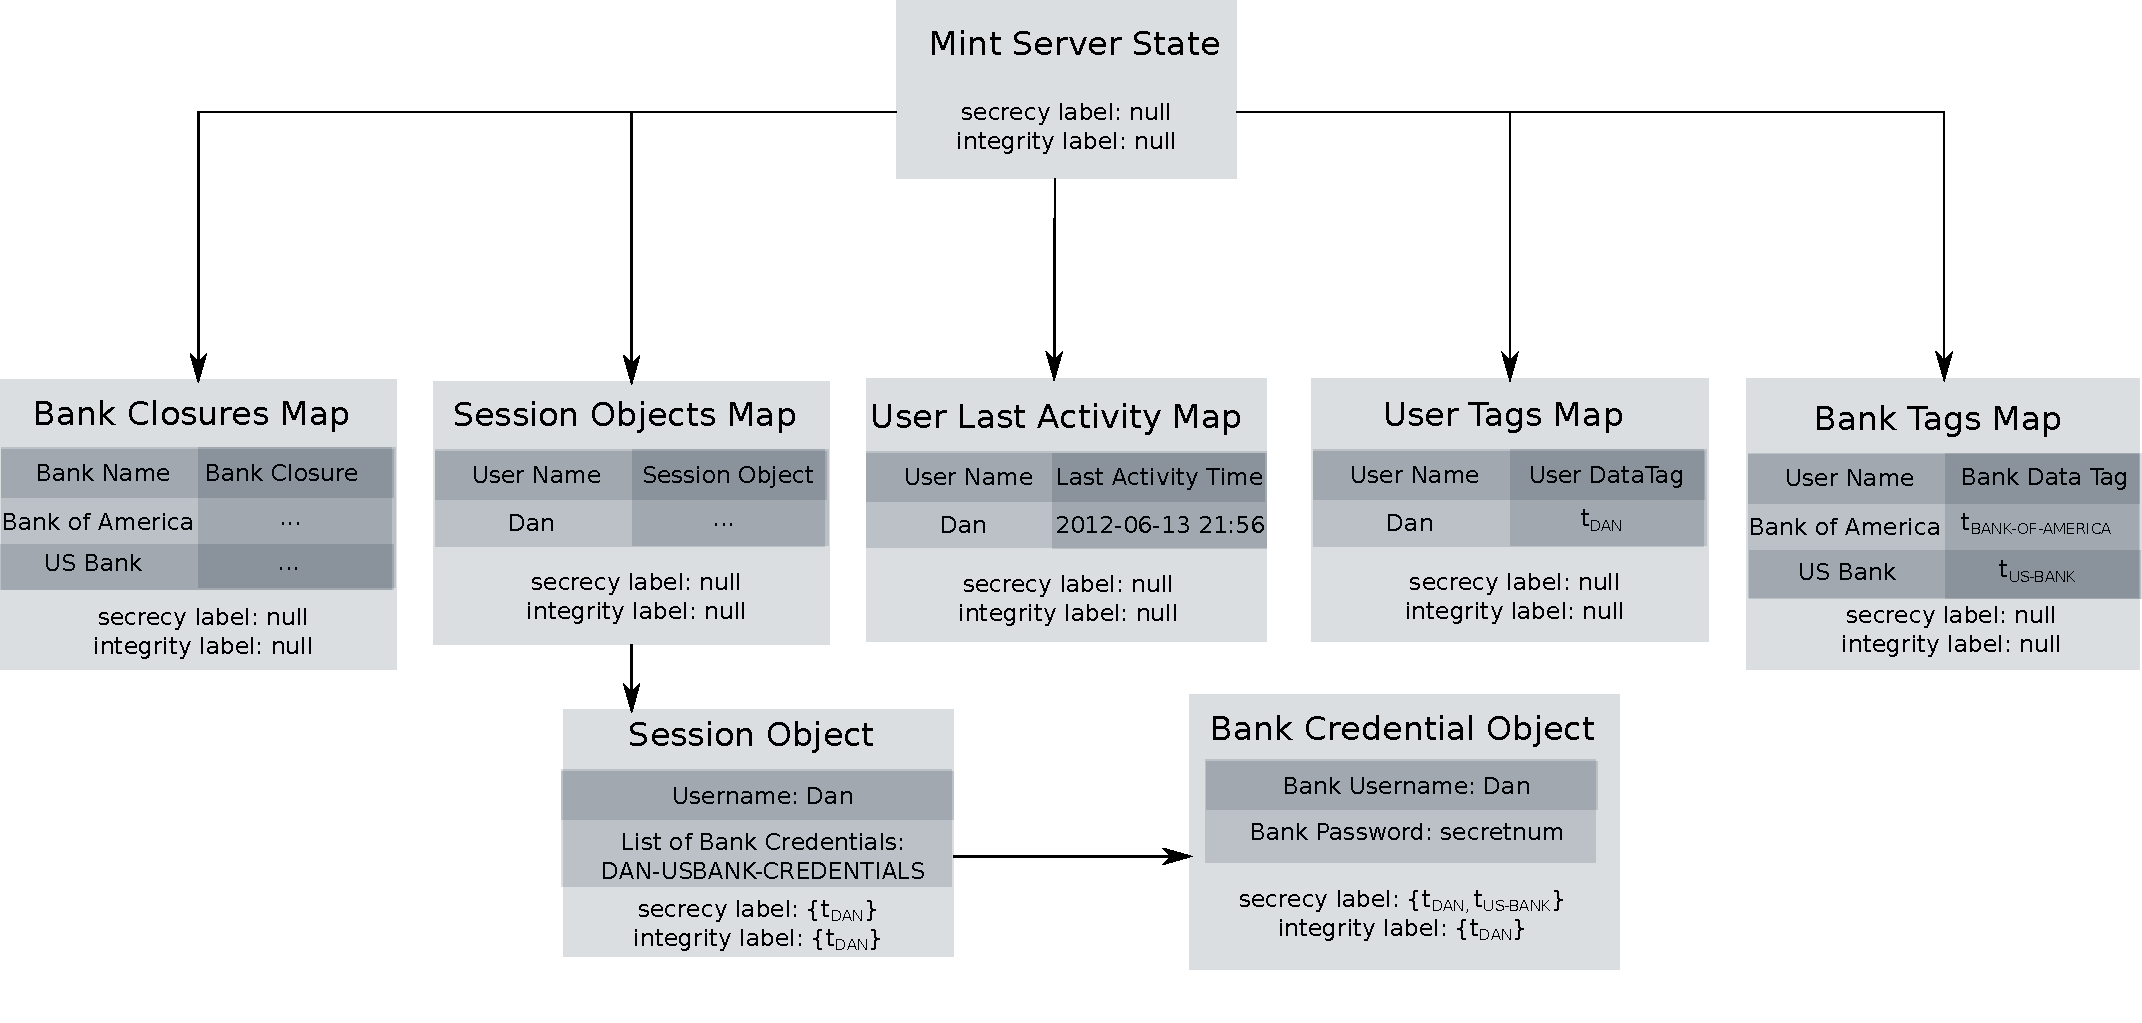
\includegraphics[width=\textwidth,height=\textheight,keepaspectratio]{figures/mint-shared-state}
\caption{Mint shared state objects. This diagram builds on the example presented in Figure \ref{fig:mint-fs}. Bob's session had timed out, and no session object or last activity time is stored for his username.}
\label{fig:mint-ss}
\end{figure}

The application uses Aeolus shared memory objects for storing session state for users and bank closures.

To allow for quick responsiveness to user requests, the application stores some key information in shared memory. Figure \ref{fig:mint-ss} diagrams the different shared memory object, their relations what information they store.

A \emph{Mint Server State} object that has null labels is stored as the Aeolus \emph{root} object and contains the following objects:

\begin{description}
  \item[Bank Closures Map] \ \\
    A bank closure is used to retrieve user
    information from a bank. The bank closure
    is authoritative for the tag of the bank
    it is working for. A bank closure has null
    labels.
    This object maps each bank name 
    to a bank closure, and has null labels.
  \item[Session Objects Map] \ \\
    This object maps a username to a session 
    object.
    A \emph{session object} contains session 
    information about a user. It also contains
    a list of \emph{bank credential} objects,
    one for each bank a user has registered 
    for, as well as the user's Principal ID
    (PID). 
    A \emph{session object} has the 
    \emph{USER-DATA} tag in both its labels.
    A \emph{bank credential} object contains 
    the user's username and password for that
    particular bank. It has a \emph{BANK-DATA}
    tag and a \emph{USER-DATA} tag in its 
    secrecy label, and a \emph{USER-DATA} tag
    in its integrity label.
  \item[User Tags Map] \ \\
    The application stores the tag for each user 
    that has an active session, this allows the 
    application server to access session objects 
    with the user tag in their label. User tags 
    are stored as a mapping from username to tag.
    This object has null labels.
  \item[Bank Tags Map] \ \\
    Bank tags are important to store in memory to 
    allow for quick server response time. They are 
    stored as a map from bank name to bank tag.
    This object has null labels.
  \item[User Last Activity Map] \ \\
    The time of a user's last activity 
    is used to identify which users
    are still active. This information is stored 
    as a mapping from username to last activity 
    time.
    This object has null labels.
\end{description}

\section{Implementation}

The application server runs on a VN, and receives user requests via RPC. Users can sign up, login, logout, register a bank and retrieve statistics. A typical flow of RPC calls is shown in figure d. 

At startup, the system registers a number of banks. These are the banks which the users can later add accounts for on their Mint account. The system is now ready to accept users.

Users can register to the Mint service through a \emph{signUp} RPC call:

\begin{description}
  \item[\emph{signUp(username, password)}] \ \\
    Signs up a new user with the username as 
    \emph{username} and password as \emph{password}. 
    If \emph{username} is available, associates 
    those credentials with a newly-created user data 
    tag and a newly-created principal ID,
    then stores all this information on disk under
    a new user directory, as per the file system
    hierarchy described in section 
    \ref{sec:mint-fs}. The system
    also stores the newly created tag in the 
    \emph{User Tags Map}.
    Throws an exception if this \emph{username}
    is already used.
\end{description}

Users can then log in to modify their account and retrieve their information using the following RPC call:

\begin{description}
  \item[\emph{login(username, password)}] \ \\
    Authenticates a user, and if successful, 
    stores their information in a session 
    object, and updates their last activity
    time using the shared memory objects
    described in section \ref{sec:mint-smo}.
    The system authenticates the 
    credentials by calling an 
    \emph{authentication closure}, which 
    adds the All User Data tag, 
    verifies the credentials, declassifies 
    and terminates if the \emph{username} and
    \emph{password} are correct, throws 
    an exception otherwise.
\end{description}

Once a user logs in, they only have to include their \emph{username} in persuing requests to carry out different actions. In each of the following RPC calls, authentication is carried out by checking if the provided \emph{username} has a session that has not timed out yet (there is a last activity time associated with a session, and thus must not be older than a certain amount of time, e.g. 15 minutes).

\begin{description}
  \item[\emph{addBank(username, bankName, bankUsername, bankPassword)}] \ \\
    Registers the specified bank 
    for the specified username with the given 
    credentials.
    This request writes a \emph{user-bank-creds} 
    file to disk, with the tag of
    the user in its integrity label, and the 
    tag of the user and that of the bank
    in its secrecy label.
  \item[\emph{downloadTransactions(username)}] \ \\
    This action connects to each bank the 
    user has registered for their account, 
    downloads the latest transactions for the user, 
    processes them, and returns the result.
    The RPC thread uses the closure of the bank to
    connect to the bank and declassify the 
    information returned. The thread then
    adds a user tag to it's secrecy label, 
    and uses a reduced authority call to 
    the public principal to process the information; 
    this ensures that information
    cannot be leaked while it is being
    processed
    \footnote{One can imagine that the 
    information is being processed by a different
    application in the system, 
    using this technique means our application 
    does not have to trust that 
    application.}. 
%    Figure x shows a code sample.

%  \item[\emph{attack(attacker, victim)}] \ \\
%    \emph{Attacks} the uer specified by \emph{victim}. 
%    This request aims to simulate a bug 
%    in the appliction that mistakingly 
%    delegates the victim's 
%    data tag to the attacker's principal.
%    This user action is useful for testing 
%    and auditing purposes, as explained later
%    in this chapter.

  \item[\emph{logout(username)}] \ \\
    Terminates the user's session, removing 
    their information from shared memory.
  \item[\emph{removeBank(username, bankName)}] \ \\
    Removes the specified bank from a user's account.

\end{description}

\noindent
For each RPC call, the thread handling the call starts running on behalf of \emph{P$_{MINT}$}, and then reduces its authority as soon as possible to avoid errors leading to information leakage. For example, in \emph{downloadTracations}, after authenticating the user, the thread reduces its authority to run on behalf of the users principal, then processes the downloaded information on behalf of \emph{P$_{PUBLIC}$} and then returns.


\section{System Security}

The use of a \emph{username} in the implementation of the RPC calls defined above to identify which user invoked those calls creates a vulnerability in our system. Alice could send a \emph{downloadTransactions(``Bob'')} request, and because the information is being sent outside the Aeolus system, the information in the reply would have null labels, and hence Alice could access Bob's information.

Another problem that comes up is related due to the assumption that the user is connecting from another Aeolus node. If this was not the case, i.e. the requests are coming from outside the Aeolus system, sensitive information would be exposed over the network (e.g. the user's Mint credentials), which wouldn't happen for RPCs within the Aeolus system because those are encrypted\footnote{Requests coming from outside the system could be RPC or HTTP requests.}.

Both issues can be resolved by using standard cryptography mechanisms to encrypt and authenticate external communication. For example, encrypting all requests and replies coming in and out of the system and, in addition, sessions can be identified by unguessable temporary session-ids, and, those session-ids would be used to authenticate future requests in that session.
